\section{Attack Description}\label{sec:attack}

\begin{figure}
  \centering
  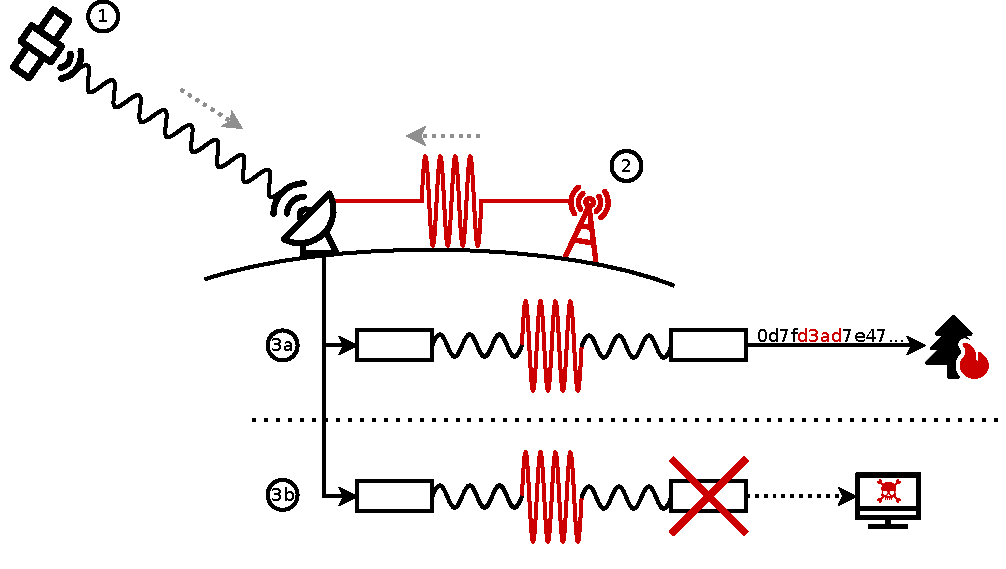
\includegraphics[width=\columnwidth]{diagrams/attack_illustration.pdf}
  \caption{An illustration of the attacks described in this paper. The attacker is indicated in red. 1)~The satellite broadcasts a signal; 2)~A ground-based attacker injects a crafted signal, overshadowing the legitimate signal and resulting in one of two scenarios; 3a)~The victim receiver decodes the attacker-controlled data, poisoning derived datasets; 3b)~The injected signal exploits vulnerabilities in the protocol decoders, resulting in denial of service or arbitrary code execution.}
  \label{fig:attack-illustration}
\end{figure}

Successfully attacking a downlink satellite system requires the attacker to reliably overshadow an active wireless communications channel, injecting a custom radio signal into the receiver.
The injected signal is designed to either, as depicted in Figure~\ref{fig:attack-illustration}, affect the decoded data or exploit processing stages in the decoding pipeline.
By affecting the decoded data, the attacker can either poison satellite-derived datasets, such as Earth observation data, or manipulate live sessions such as internet traffic.
By instead creating malformed packet headers, attackers can also seek to manipulate control flow in the decoding software and exploit potential vulnerabilities.

We proceed to discuss the key physical and protocol layer factors in performing a successful overshadow.
We demonstrate and assess the effects against real-world systems in Section~\textbf{TODO}.

\subsection{Physical layer considerations}

At the physical layer, the attacker must emit a sufficiently high gain interfering signal such that the receiver no longer decodes the original signal.
Achieving this in the real world is non-trivial, since the equipment setup must be operate at the correct radio frequency, transmission power, and signal polarity.

\subsubsection{Radio frequency}

Historically, securing satellite wireless channels has not been a priority for satellite operators, which prioritise system robustness over security guarantees~\textbf{TODO: mention the FUNcube email from Josh}.
It was also assumed that the equipment required to eavesdrop and inject messages is highly specialised and difficult to access.
However, recent software-defined radio (SDR) hardware can transmit and receive signals cheaply up to the UHF and VHF frequencies (up to 6GHz)~\textbf{TODO: cite HackRF}, lowering the barrier to entry for injection attacks.

Insecure satellite signals in this range are therefore most affected; eavesdropping is possible with only an SDR and cheap television equipment~\cite{pavur2020tale}.
We demonstrate that these signals are also the easily overshadowed, requiring only a simple amplifier and antenna setup as used in amateur radio.
Targetable systems include geostationary satellite internet providers, GNSS, television, and some communications satellites~\cite{esa_satellite_bands}.

However, the majority of military and communications satellites downlink data in the X-band (8-12GHz), Ku-band (12-18GHz), or the Ka-band (26-40GHz).
Since SDRs can't output in these frequencies, overshadowing requires upconverting and amplifying the signal with special-purpose high frequency radio equipment.
Additionally, since the higher frequencies are more easily blocked by physical materials and less diffracted in the atmosphere, the attacker has to achieve line-of-sight with the receiver station.
Off the shelf radio equipment for this is highly expensive; Endurosat sells the upconverter and transmitter for $22,800$ EUR~\cite{endurosat:xbandtransmitter}, and a compatible antenna for $6,400$ EUR \cite{endurosat:xbandantenna}.

In Section~\textbf{TODO} we discuss how an attacker can design a custom transmission setup covering these frequency ranges at a much lower cost.

\subsubsection{Transmission power}

Antennas intended for space communications tend to be highly directional, amplifying signals within a certain beam, and attenuating out of beam signals.
Each antenna type has a unique gain pattern; monopole antennas, Yagi antennas, and parabolic dishes attenuate out-of-band signals considerably differently.
Therefore, ground-based attackers transmitting out of beam must overcome the attenuation through sufficiently high gain.
However, if the attacker transmits at an excessively high power, the victim receiver will be saturated and unable to decode the signal.

Therefore, the attacker must transmit at the correct power such that the legitimate signal is overshadowed, but the receiver is not saturated.
In Section~\textbf{TODO}, we determine how the attacker can establish this through modelling and experimental evaluation of several antenna types.

% TODO: saturation graph?

\subsubsection{Signal polarity}

Electromagnetic waves can either be linearly or circularly polarised; the polarity of satellite communications varies between each satellite system.
As a result, incorrectly polarised signals are attenuated, and correctly polarised signals are received.
Therefore, the attacker must ensure that the emitted signal is of the correct polarity.

Although the attacker can transmit at different polarities by changing or rotating the transmission antenna, effective overshadowing also requires correct alignment with the receiving system.
There are multiple ways of establishing the correct polarity even if the satellite isn't publicly documented; the attacker can inspect the receiver or attempt to receive the signals themselves.

The experiments in Section~\textbf{TODO} are designed to establish the importance of aligning with the receiver polarisation, given real world effects such as multipath propagation.

\subsection{Protocol layer considerations}

% TODO: are these really worth discussing?

In a successful signal injection attack, the injected data must either accepted and decoded by the victim, or be malformed to exploit a vulnerability in the decoder.

\subsubsection{Cryptography}

Robust cryptgraphy can prevent all forms of signal injection attacks by guaranteeing data confidentiality, integrity, and authenticity.
However, many real-world satellite downlink transmissions are either unencrypted, only partially encrypted, or are encrypted using a leaked key/weak algorithm.

Systems where the receiver software is insecurely implemented are also vulnerable.
For example, recent academic work has shown that that several major consumer satellite internet terminals are designed to handle both unencrypted and encrypted data.
In these scenarios, an attacker doesn't need to break the cryptography to achieve message decoding.

\subsubsection{Data integrity}

The physical layer characteristics of satellite transmissions results in highly noisy channels which are prone to bit flips.
As a result, SATCOM links generally include integrity checks such as checksums.
Although not providing theoretic security guarantees, such measures do prevent simple bit-flipping attacks through injecting noise.

\subsubsection{Timing}

Finally, since many satellite data transmissions form continuous streams of data, attackers injecting signals must ensure that the injected data is continuous with the existing transmissions.

\begin{comment}
% reactive jamming discussion - put later
Depending on their goals, the attacker can either generate the signal to be injected beforehand or in real time.
Generating the data beforehand does not require a receiver, only hardware capable of transmitting, but does require that the attacker generate their own data or find relevant prior broadcasts to manipulate and replay.
Alternatively, with the addition of their own receiver dish, an attacker can receive the broadcast themselves and process it in real time to add artifacts or mask specific properties of the signal.

% Call forward to the evaluation section
In the case of FIRMS, the satellite-derived dataset is a map of active forest fires, each with coordinates and a confidence value.
The dataset is derived primarily from the infrared bands of the MODIS sensor, which can reveal hotspots on the surface.
We consider the scenarios of injecting ficticious forest fires and masking existing ones, both in the pre-prepared and real-time setups.
We also perform a security analysis of the decoding software itself, demonstrating how vulnerabilities in the protocol handling can lead to denial of service and arbitrary code execution upon reprocessing.



\subsection{Affecting satellite-derived datasets}

To affect a derived dataset such as forest fire detection, the attacker needs to inject a signal that decodes to the desired raw data.
This data must target the algorithm responsible for generating the desired dataset, causing it to misclassify its input.
This leads to effects such as the detection of ficticious forest fires, and the masking of existing ones. %TODO: rephrase? masking isn't really the opposite of detection

Where the raw data is used for generating multiple derived datasets, the attacker may need to be careful to ensure that the injected data sufficiently resembles legitimate data to avoid detection. % TODO: rewrite - data, data, data...
For example, the MODIS data is used to generate color-corrected images of the Earth's surface, with the forest fire data rendered on top.
If the images appear out of sequence, distorted, or not like the Earth's surface at all, the downstream services which rely upon the data are unlikely to trust it.

As a result, we assume that for this case the attacker begins with instrument data that is sufficiently close to the original signal.
The means for obtaining such data include replaying old data, generating new convincing data, or running the attack setup in real time.
% These different approaches, and their advantages and drawbacks, are discussed in Section~\ref{sec:evaluation}.

% Getting the images to not appear distorted can itself be a challenge
% We can show the scan line problem for this

% TODO: some diagram of the packet and its fields?

Once this data has been obtained, the attacker needs to determine how to manipulate the instrument data, and then reencode it according to the packet protocol.
Each satellite system and instrument is likely to use its own custom protocol for its data channel.
In the case of MODIS, the format consists of an extension to the CCSDS \textit{Space Packet Protocol} (SPP), the dominant network layer protocol for space and satellite systems~\cite{modisDescription},p177.

After the primary header, a secondary header is used to encode timing information alongside information about the packet type and location in the overall image.
The sensor readings are represented as a densely packed array of 12-bit words within the data zone, with a trailing checksum.
Each value represents the intensity of light incident to the sensor of a specific frequency band, which is indicated by the position of the word within the array~\cite{modisDescription},p183-189.

FIRMS derives its dataset from the \textit{MODIS Active Fire Product Science Processing Algorithm} (MOD14\_SPA), which primarily uses the bands of 4 and 11 micrometer wavelengths in the infrared spectrum to detect hotspots.
Therefore, in order to manipulate the detected fires whilst leaving the visible images untouched, the attacker only needs to affect the values in these channels and recalculate the checksum.
%other bands are used are used for the rejection of false positives, and could theoretically be manipulated for finer-grained control.

Once the falsified data has been created, the attacker needs to reencode it according to the packet protocol used.
For Terra and Aqua, the MODIS data is already in the network layer protocol SPP, which must then be acked into data link layer frames for broadcast.
Satellites such as those in the EOS fleet implement a custom data link layer protocol, fine-tuned to their operational requirements.

\begin{figure*}
    \centering
    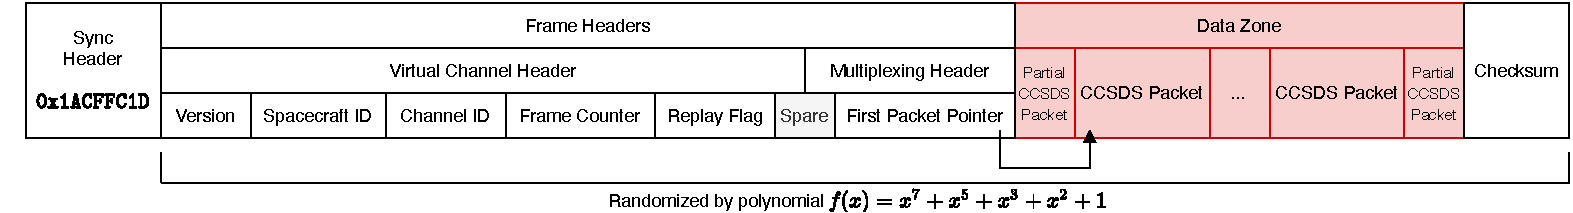
\includegraphics[width=\textwidth]{diagrams/cadu_diagram.pdf}
    \caption{Layout of data within a Channel Access Data Unit (CADU). The section marked in red can contain arbitrary attacker-specified data.}
    \label{fig:cadu_diagram}
\end{figure*}

Terra and Aqua make use of the custom \textit{Channel Access Data Unit} (CADU) protocol shown in Figure~\ref{fig:cadu_diagram}, a fixed-length frame structure containing a synchronising header and checksum~\cite{spaceGroundAqua},p32.
The CADU is optionally Viterbi encoded (XORed with a fixed polynomial) to prevent desynchronisation during long runs of the same symbol.

Finally, the attacker must note that the decoder is likely to perform additional checks on top of adhering to the known standards.
As a result, the injected data may be rejected if, for example, it doesn't specify the correct version number in the header, or is of an unexpected length.

%Since Earth-observing satellites often contain multiple instruments, and need to commuicate a mixture of scientific, engineering, and housekeeping information, a packet-based structure is chosen.
%SPP supports this through Application IDs in the primary header; each instrument is given a unique ID, allowing the data from each to be multiplexed onto the same downlink.

% In the case of publicly documented satellites, this is easier
% However, even proprietary satellites tend to use certain standard protocols in order to make this easier
% James Pavur's work on looking at data in DVBS/2 is related - you can scan the satellite's data to try and determine what its type is



\subsection{Exploiting downlink processing stages}

\begin{figure}
    \centering
    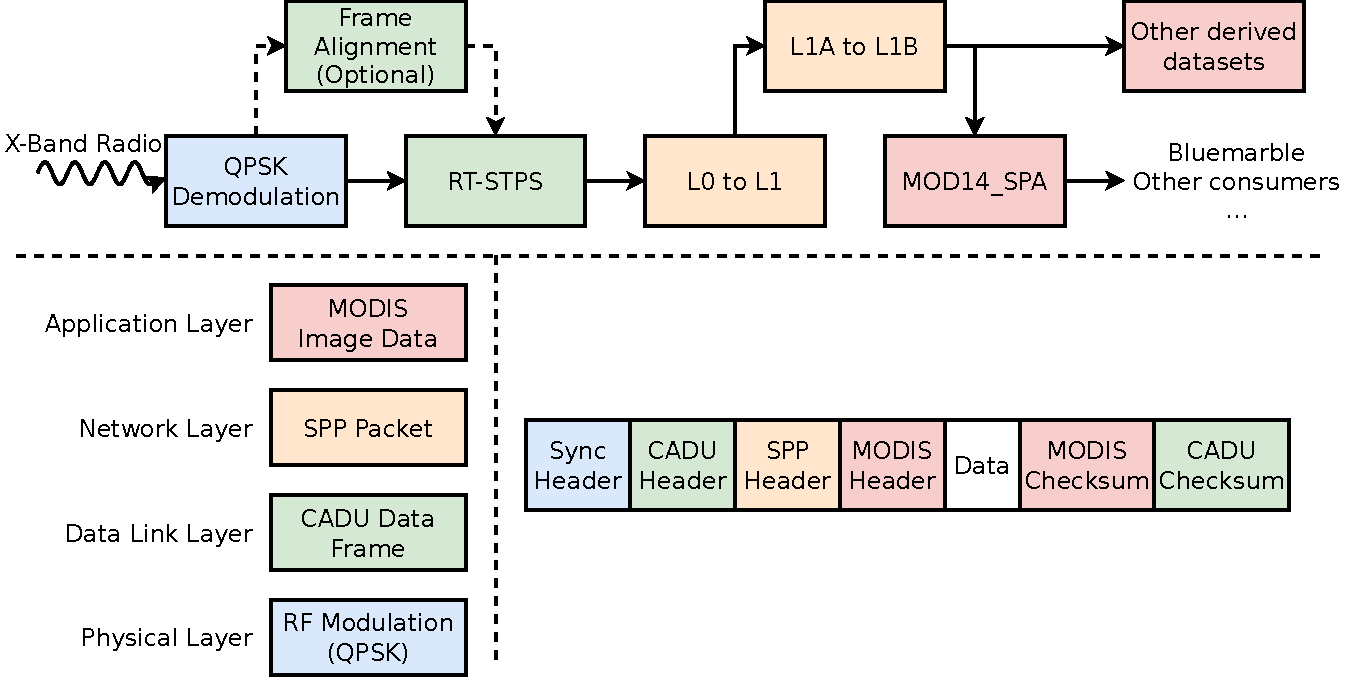
\includegraphics[width=\linewidth]{diagrams/attack_types.pdf}
    \caption{Illustration of the steps involved in processing MODIS image data and derived datasets, as well as the packet structure and layer within the network stack.}
    \label{fig:attack_types}
\end{figure}

% Describe not specific attacks, but the pipeline itself

% NB: we haven't really explained how the different parts of the protocol relate to parts of the packet, and the available attacks

However, in addition to manipulating the instrument data itself, attackers are also able to change protocol-specific fields within the packet headers.
These fields are parsed and used by the initial stages of the processing pipeline to validate and error correct the downlinked signal, and demultiplex and extract the data into an intermediate structure.
As a result, attackers can potentially exploit these early pipeline stages through crafting packets to trigger vulnerabilities.

As a case study we consider NASA's \textit{International Planetary Observation Processing Package} (IPOPP), a software distribution for decoding and processing EOS data.
The software in IPOPP contains protocol decoding stages alongside the satellite-derived dataset generation algorithms.
In particular, the \textit{MODIS Level-1 Science Processing Algorithm} (MODISL1DB\_SPA) is responsible for decoding SPP packets with the MODIS secondary header into the \textit{Heirarchical Data Format} (HDF)~\cite{modisL1DB}.
A summary of the entire pipeline can be found in Figure~\ref{fig:attack_types}.
With a long history going back to the early EOS satellites, the overall system has grown to be incredibly complex, with many interrelating dependencies and execution pathways.
Through overshadowing the signal, an attacker can deliver arbitrary bytes to these processing stages, which were not designed with untrusted input data in mind.

In Section~\ref{sec:evaluation} we consider the effect of a modern adversary against this system.
We demonstrate how the complex execution pathway includes input data being passed between several different processing applications unsafely.
Ultimately, this results in the creation of a payload which gets inserted into the intermediate data structure, and may be triggered by a future reprocessing step.

However, IPOPP is also potentially exploitable due to other well-known vulnerabilities.
Part of the complexity of the system is due to its high number of dependencies, many of which come pre-bundled with the source code.
These dependencies include outdated libraries with documented CVEs (Common Vulnerabilities and Exposures) which haven't been patched.
For example, at the time of writing, MODISL1DB\_SPA comes bundled with HDF5 v1.12.0, which has 11 active CVEs.

% Do I need to explain here exactly what processing stages are involved?

% The code is distributed mixed in with pre-compiled binaries and libraries which are required to make the system work
% Interestingly, Too old for log4shell, for which it is not patched

The extent to which other processing software may be vulnerable to similar attacks is hard to quantify.
However, satellite operators should be aware that similar systems, which may not have been designed to be resilient to untrusted input data, could be exploitable through similar techniques.
\end{comment}
